\documentclass[a4paper,11pt]{report}
\usepackage[sc]{mathpazo}
%\usepackage[light,firsttwo,outline,bottomafter]{draftcopy}
%\usepackage{srcltx}
\usepackage{anysize} % Soporte para el comando \marginsize
\marginsize{1.2cm}{1.2cm}{1cm}{1cm}
\usepackage{amsfonts}
\usepackage{amssymb}
\usepackage[latin1]{inputenc}
\usepackage[english,spanish]{babel}
\usepackage{amsmath}
\usepackage{multicol} 
\columnsep=7mm
\usepackage{latexsym}
\usepackage{mathrsfs}
\usepackage{bigints}
\usepackage{indentfirst}
\usepackage{graphicx}
\usepackage{enumitem}
%\usepackage{hyperref}

\usepackage{times}



%\usepackage{xcolor}
%\usepackage{pgfplots}
%\usepackage{tikz}

%
%\definecolor{bblue}{HTML}{4F81BD}
%\definecolor{rred}{HTML}{C0504D}
%\definecolor{ggreen}{HTML}{9BBB59}
%\definecolor{ppurple}{HTML}{9F4C7C}


\setlength{\paperwidth}{216mm} \setlength{\paperheight}{230mm}
\setlength{\textwidth}{39pc} \setlength{\textheight}{57.5pc}
\setlength{\topmargin}{-1.5cm} \setlength{\oddsidemargin}{-0.5cm}
\setlength{\evensidemargin}{0.9cm}
%\setlength{\footskip}{-0.3cm}

\newcommand{\ds}{\displaystyle}
\newcommand{\normal}{\triangleleft \,}
\newcommand{\tx}{\textrm}
% \linespread{1.2} \sloppy


\newcommand{\Z}{\mathbb{Z}}
\newcommand{\N}{\mathbb{N}}
\newcommand{\R}{\mathbb{R}}
\newcommand{\PR}{\mathbb{P}}
\newcommand{\e}{\rightarrow}
\newcommand{\bi}{\Leftrightarrow}
\newcommand{\com}{\mathbb{N} \bi}
\newcommand{\fu}{f:\N \e \R}
\newcommand{\ba}{\backslash}
\newcommand{\Q}{\mathbb{Q}}


\newcommand{\calP}{\mathcal{P}}
\newcommand{\calF}{\mathcal{F}}
\newcommand{\calL}{\mathcal{L}}


\newcommand{\ovl}{\overline}
\newcommand{\ora}{\overrightarrow}
\newcommand{\ola}{\overleftarrow}
\newcommand{\olra}{\overleftrightarrow}{\tiny }
\newcommand{\ula}{\underleftarrow}
\newcommand{\ura}{\underrightarrow}


\newcommand{\inner}[2]{\langle{#1},{#2}\rangle}


\begin{document}
\begin{center}
	{\LARGE\textbf {Preguntas de Introducci\'on a los Procesos Estoc\'asticos}}
\end{center}

\setlength{\unitlength}{1in}

\begin{picture}(6,.1) 
\put(0,0) {\line(1,0){6.25}}         
\end{picture}
\vspace{0.8cm}

\vspace{0.2cm}
	
	\renewcommand{\arraystretch}{2}
	
	\vskip.25in
	
	\noindent {\Large \textbf{Lista de Problemas}} 
	
	\vskip.25in

%\begin{multicols}{1}

 \vspace{0.3cm}
 
\begin{enumerate}
\item Suponiendo que $f:[0,1] \rightarrow [0,1]$ es una funci\'on continua. Muestra un \texttt{m\'etodo probabilistico } para evaluar $\bigintsss_{0}^{1}f(x) dx$, usando la \textit{Ley Fuerte de los Grandes N\'umeros}.

\item 

\begin{enumerate}
	\item Se lanza una moneda en repetidas ocasiones, las caras  que se producen en cada lanzamiento tienen probabilidad $p$. Encuentra la funci\'on generadora  de probabilidad del n\'umero $T$ de lanzamientos antes de que $n$ caras  hayan  aparecido por primera vez.
	\item Encuentra la funci\'on generadora de la funci\'on de masa binomial negativa
	
	\[
	f(k) = \binom{k - 1}{r - 1}p^r(1 - p)^{k - r}, \ \  \ k = r, r + 1, \dots
	\]
	
	donde $0 < p < 1$ y $r$ es un entero positivos. Deduce la media y la varianza.
\end{enumerate}
\item 
\begin{enumerate}
	\item Sean $X_2, X_3, \dots $ variables aleatorias independientes tal que
	\[
	\PR(X_n) = \PR(X_n = -n) = \frac{1}{2n \log n},\ \ \PR(X_n = 0) = 1 - \frac{1}{n\log n}
	\]
	
	Muestra que esta secuencia cumple la ley d\'ebil de los grandes n\'umeros, pero no la ley Fuerte, en el sentido  que $n^{-1}\sum_{1}^{n}X_i$ converge a $0$ en probabilidad.
	\item Sean $X_1, X_2, \dots $ variables aleatorias independientes con una funci\'on densidad
	
	\[
	f(x) = \begin{cases}
	0 & \text{si}\ \ \ \vert x \vert \leq 2,\\
	\frac{c}{x^2\log \vert x \vert } & \text{si}\ \ \vert x \vert > 2
	\end{cases}
	\]
	
	donde $c$ es una constante. Muestra que $X_i$ no tiene media, pero $n^{-1}\sum_{1}^{n}X_i \rightarrow 0$ en probabilidad cuando $n \rightarrow 0$.
\end{enumerate}

\item 

\begin{enumerate}
	\item Sea $X_1, X_2, \cdots $ una secuencia de variables aleatorias Bernoulli con param\'etro $p$, independientes e id\'enticamente distribuidas. Prueba que para un $\epsilon > 0$, se tiene
	
	\[
	\PR\Bigl( \Bigl\vert \frac{S_n}{n} - p \Bigr\vert \geq \epsilon\Bigr) \leq \frac{1}{4n\epsilon^2}
	\]
	
	donde $S_n = X_1 + X_2 + \cdots X_n$.
	\item Sea $X$ una variable no negativa. Prueba
	
	\[
	\mathbb{E}(X) \leq [\mathbb{E}(X^2)]^{\frac{1}{2}} \leq [\mathbb{E}(X^3)]^{\frac{1}{3}}\leq \dots
	\]
	
	\item Sea $X$ e $Y$ variables aleatorias independientes, con media $0$ y varianza $1$ y una funci\'on \mbox{generadora} de momentos $M(t)$. Si $X +Y$ y $X -Y$ son independientes, muestra que
	
	\[
	M(2t) = M(t)^3M(-t)
	\]
	
	y deduce que $X$ e $Y$ tienen una distribuci\'on normal con  media $0$ y varianza $1$ .
\end{enumerate}
\item 

Considera un Proceso de Poisson, con param\'etro $\lambda$ y sea $N(G_i)$ denota el n\'umero de llegadas del proceso durante el intervalo $(t_i, t_i + c_i ]$. Supongamos que tenemos $n$ intervalos, $i = 1,2, \cdots, n$ mutualmente disjuntos. Denotemos la uni\'on de esos intervalos por $G$ y su longitud total $c = c_1 + c_2 + \cdots c_n$. Dado $k_i \geq 0$ y con $k_1 + k_2 + \cdots + k_n$, determina

\[
\PR\Bigl( N(G_1)= k_1, N(G_2) = k_2, \dots, N(G_n) = k_n | N(G) = k\Bigr).
\]

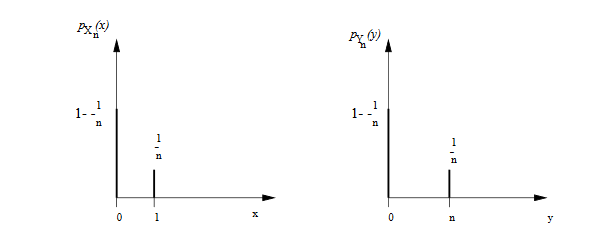
\includegraphics[scale=0.8]{p1}

\item  Sean $X_n$ e $Y_n$ con distribuciones, mostradas en el anterior gr\'afico

\begin{enumerate}
	\item Encuentra la media y la varianza de $X_n$ y $Y_n$.
	\item ?` Qu\'e nos dice la desigualdad de Chebyshev acerca de la convergencia de $X_n$ e $Y_n$?.
	\item ?` Es $Y_n$ convergente en probabilidad?. ?` Cu\'al es el valor si es que es convergente en \mbox{probabilidad}?.
	\item ?`Si una secuencia de variables aleatorias converge en probabilidad a $a$, entonces la secuencia de valores esperados converge tambi\'en a $a$?. Prueba o da un contraejemplo.
	
	\vspace{0.2cm}
	
	
	Una secuencia de variables aleatorias se dice que converge a un n\'umero $c$ en \textit{media cuadr\'atica}, si
	
	\[
	\lim_{n \rightarrow \infty}\mathbb{E}[(X_n - c)^2] = 0
	\]
	
	
	\item Usa la desigualdad de Markov, para probar que la cobvergencia en media cuadr\'atica implica convergencia en probabilidad.
	\item Da un ejemplo que muestra que la convergencia en probabilidad no implica convergencia en media cuadr\'atica.
\end{enumerate}





\item  Resuelve lo siguiente

\begin{enumerate}
	\item Prueba que se cumple  $n! \sim \sqrt{2\pi n}n^ne^{-n}$ o lo que es lo mismo
	
	\[
	\lim_{n \rightarrow \infty}\dfrac{n!}{\sqrt{2\pi n}n^ne^{-n}}
	\]
	
	\item Sea $\{X_1, X_2, \dots  \}$ una secuencia de variables aleatorias normal est\'andar independientes. Sea $S_n = X_1^2 + X_2^2 + \cdots X_n^2$. Encuentra
	
	\[
	\lim_{n \rightarrow \infty}\mathbb{P}(S_n \leq n + \sqrt{2n}).
	\] 
\end{enumerate}

\item  Si $X$ e $Y$ tienen funci\'on generadora de probabilidad conjunta

\[
G_{X,Y}(s, t) = \mathbb{E}(s^Xt^Y) = \frac{\{1 - (p_1 + p_2)\}^n}{\{1 - (p_1s + p_2t)\}^n}, \ \  \text{donde}\ \ p_1 + p_2 \leq 1
\]

encuentra las funciones de masa marginales de $X$ e $Y$ y la func\'on  de masa de $X + Y$. Encuentra la probabilidad generadora condicional $G_{X|Y}(s | y) = \mathbb{E}(s^X| Y = y)$ de $X$ dado que $Y = y$. 

\item  Sea una secuencia $X_1, X_2, \dots$ de variables aleatoria binarias tomando valores en el \mbox{conjunto} $\{0, 1\}$. Sea $Y$ una variable aleatoria continua que toma valores en $[0, 1]$. Relacionamos $X$ e $Y$ \mbox{asumiendo} que $Y$ es el n\'umero real cuya representaci\'on binaria es $0.X_1X_2X_3\dots$, es decir

\[
Y = \sum_{k = 1}^{\infty}2^{-k}X_k
\]

\begin{enumerate}
	\item Suponiendo que $X_i$ forman un proceso de Bernoulli con param\'etro $\frac{1}{2}$. Muestra que $Y$ es \mbox{distribuida} uniformemente (considera la probabilidad del evento $(i - 1)/2^k < Y < i/2^k$, donde $i$ y $k$ son enteros positivos).
	\item Suponiendo que $Y$ es distibuida uniformemente. Muestra que las $X_i$ forman un proceso de \mbox{Bernoulli} con param\'etro $\frac{1}{2}$.
\end{enumerate}
\item  

Sea el n\'umero de \'exitos en $n$ pruebas de Bernoulli, donde la probabilidad de \'exito en cada prueba es $p = \frac{1}{2}$. Proporciona un valor n\'umerico para el l\'imite cuando $n$ tiende al infinito para cada una de las siguientes expresiones

\begin{itemize}
	\item $\PR(\frac{n}{2}- 10 \leq S_n \leq \frac{n}{2} +  10)$
	\item $\PR(\frac{n}{2} - \frac{n}{10} \leq S_n \leq \frac{n}{2} + \frac{n}{10} )$
	\item $\PR(\frac{n}{2} - \frac{\sqrt{n}}{2} \leq S_n \leq \frac{n}{2} + \frac{\sqrt{n}}{2} )$
\end{itemize}

\item 
\begin{enumerate}
	\item Sean $X_1, X_2, \dots, X_n, X_{n + 1}, \dots, X_{2n}$ variables aleatorias id\'enticamente distribuidas e \mbox{independientes}.
	Encuentra
	
	\[
	\mathbb{E}[X_1|X_1 + X_2 + \dots, X_n = x_0],
	\]
	donde $x_0$ es una constante.
	
	\item Definimos
	
	\[
	S_k = X_1 + X_2 + \dots + X_{k}, \ \ \  1 \leq k \leq 2n.
	\]
	
	Encuentra 
	
	\[
	\mathbb{E}[X_1| S_n = s_n, S_{n + 1} = s_{n + 1}, \dots S_{2n} = s_{2n}]
	\]
	
	donde $s_n, s_{n + 1}, \dots, s_{2n}$ son constantes.
\end{enumerate}

\item  Sean $X$ e $Y$ variables aleatorias tomando valores enteros positivos, tal que

\[
\PR(X = k| X + Y = n) = \binom{n}{k}p^k(1 - p)^{n - k}
\]

para alg\'un $p$ y todo $0 \leq k \leq n$. Muestra que $X$ e $Y$ tienes distribuciones de Poisson.

\item 

\begin{enumerate}
	\item Prueba que $\mathbb{E}\{\mathbb{E}(X | Y, Z)| Y  \} = \mathbb{E}(X| Y)$.
	\item Supongamos que $\mathbb{E}\vert X^r \vert <  \infty$, donde $r >0$. Deduce que $x^r\PR(\vert X \vert  \geq x) \rightarrow 0$ cuando $x \rightarrow \infty$. De igual forma si $x^r\PR(\vert X \vert  \geq x) \rightarrow 0$,  cuando $x \rightarrow \infty$  donde $r \geq 0$, muestra que $\mathbb{E}\vert X^s \vert < \infty $ para $0 \leq s <  r $.
	\item Sea $X$ una variable aleatoria que toma valores en el intervalo $[-M, M]$. Muestra que
	
	\[
	\mathbb{P}(\vert X \vert \geq  a) \geq \frac{\mathbb{E}\vert X \vert - a }{M - a}
	\]
	
	si $0 \leq a < M$.
\end{enumerate}
\item   Sea $Y_1, Y_2, \dots$ variables aleatorias independientes, id\'enticamente distribuidas que toma \mbox{valores} en $[0, \infty)$. Si se coloca $Z_0 = 0, Z_1 = Y_1, Z_2 = Y_1 + Y_2, \dots$. Si $Z_n$ es el tiempo del n-\'esima llegada a una tienda (el proceso estoc\'astico $\{ Z_n: n \in \mathbb{N}\}$) es llamado \textit{renewal process}. Sea $N_{t}$ el n\'umero de llegadas durante $(0, t]$.

\begin{enumerate}
	\item Muestra que
	
	\[
	\PR(N_t \geq n) = \PR(Z_n \leq t)
	\]
	
	para todo $n \in \mathbb{N}$ y $t \in [0, \infty)$.
	
	\item Muestra que para \textit{casi todo } $\omega$,
	
	\[
	\lim_{t \rightarrow \infty}N_t(\omega) = + \infty
	\]
	
	\item Si $Z_{N_{t}}$ es el tiempo de la \'ultima llegada antes del tiempo $t$ y $Z_{N_{t} + 1}$ es el tiempo de la pr\'oxima  llegada despu\'es  del tiempo $t$. Usa la ley fuerte de los grandes n\'umeros y el resultado anterior para probar que 
	
	\[
	\lim_{t \rightarrow \infty}Z_{N_{t}}/N_{t} = a
	\] 
	
	donde $a$ es el valor esperado de $Y$.
\end{enumerate}
\end{enumerate}

\begin{flushright}
%\\{\bfseries El profesor.}
\footnote{Hecho en \LaTeX}
\end{flushright}

\end{document}
